\documentclass{../konspekt}

\title{Elektryczność i Magnetyzm konspekt}

\begin{document}

\begin{multicols}{2}

  \section{Ładunek}

  $$
  q = n \cdot e
  $$
  n - liczba ładunków elementarnych, $e = 1.6 \cdot 10^{-19} C$

  \section{Prawo Coulomba}

  $$
  \vec{F_E} = k \cdot \frac{q_1 \cdot q_2}{r^2} \cdot \vec{r}
  $$
  gdzie $k$ to stała elektrostatyczna($\frac{1}{4\pi\epsilon_0}$,
  $\epsilon_0\approx8.854\cdot10^{-12}\frac{E}{m}$) a $q$ to ładunki.

  \section{Pole elektryczne}

  $$
  \vec{E}(r) = k \cdot \frac{|q|}{r^2} \cdot \vec{r}
  $$
  Gdzie $r$ to odległość od ładunku, a $q$ to ładunek, tworzący pole
  elektryczne.
  $$
  \vec{F_E} = q \cdot \vec{E}(r)
  $$

  \section{Prawo Gaussa}

  $$
  \oint_S E \cdot dS = \frac{1}{\epsilon_0} \int_V \rho(r) dr =
  \frac{\rho_{\text{zamknięte}}}{\epsilon_0}
  $$
  Całka po zamkniętej powierzchni $S$(gaussowskiej) z pola
  elektrycznego $E$ jest równa całce po gęstości ładunku $\rho$ w
  objętości $V$ podzielonej przez $\epsilon_0$.

  Typowo podczas rozwiązywania zadań, znajdujemy infitisemalnie małą jednostkę
  ciała $dS$ i całkujemy po powierzchni $S$ aby znaleźć całkowite pole
  elektryczne.

  Ładunek na skutek nieskończonej linii naładowanej równomiernie
  ładunkiem $\lambda$ jest równy:
  $$
  E(a) = \frac{\lambda}{2\pi\epsilon_0 a}
  $$

  \section{Potencjał elektryczny}

  $$
  E = - \nabla V
  $$
  czyli pole elektryczne jest równe gradientowi potencjału
  elektrycznego.
  $$
  F_E = qE = -q \nabla V = - \nabla U
  $$
  $U$ to energia potencjalna, a $V$ to potencjał elektryczny.
  $$
  U = qV
  $$

  \section{Kondensatory}

  $$
  C = \frac{Q}{V}
  $$
  gdzie $C$ to pojemność kondensatora, $Q$ to ładunek na
  kondensatorze, a $V$ to napięcie na kondensatorze. Kondensatory połączone
  równolegle mają pojemności sumowane:
  $$
  C_{eq} = C_1 + C_2 + \ldots
  $$
  Kondensatory połączone szeregowo mają pojemności odwrotne:
  $$
  \frac{1}{C_{eq}} = \frac{1}{C_1} + \frac{1}{C_2} + \ldots
  $$
  Energia zgromadzona w kondensatorze:
  $$
  W = \int_{0}^{Q} \frac{Q}{C} dQ = \frac{Q^2}{2C} = \frac{1}{2} C V^2
  $$

  \section{Opór elektryczny}

  $$
  R = \frac{V}{I}
  $$
  $$
  I = \frac{Q}{t}
  $$
  $R$ to opór elektryczny, $V$ to napięcie, $I$ to prąd,
  $Q$ to ładunek.

  \section{Siła Lorentza}

  $$
  F = q \cdot (E + v \times B)
  $$
  gdzie $F$ to siła Lorentza, $q$ to ładunek, $E$ to pole elektryczne,
  $v$ to prędkość ładunku, a $B$ to pole magnetyczne.

  $$
  F = q \cdot v \cdot B \cdot \sin(\alpha) = q \cdot v \cdot B =
  \frac{\mu_0 I q v}{2\pi a}
  $$

  \section{Cewka}

  $$
  B = \frac{\mu_0 I}{2\pi r}
  $$
  dla cewki o promieniu $r$ i prądzie $I$.

  \section{SEM}

  $$
  \text{SEM} = \mathcal{E} = -N \frac{d \Phi}{dt}
  $$
  gdzie SEM to siła elektromagnetyczna, $N$ to liczba zwojów, a $\Phi$
  to strumień magnetyczny.
  $$
  \Phi = BS \cos(\alpha)
  $$

  \section{Zasada prawej ręki}

  \begin{center}
    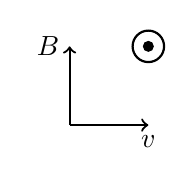
\begin{tikzpicture}
      \draw[thick,->] (0,0) -- (1,0) node[anchor=north] {$v$};
      \draw[thick,->] (0,0) -- (0,1) node[anchor=east] {$B$};

      \draw[thick] (1,1) circle (0.2);
      \fill (1,1) circle (0.07);
    \end{tikzpicture}
    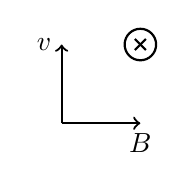
\begin{tikzpicture}
      \draw[thick,->] (0,0) -- (1,0) node[anchor=north] {$B$};
      \draw[thick,->] (0,0) -- (0,1) node[anchor=east] {$v$};

      \draw[thick] (1,1) circle (0.2);
      \draw[thick] (0.93,0.93) -- (1.07,1.07);
      \draw[thick] (0.93,1.07) -- (1.07,0.93);
    \end{tikzpicture}
  \end{center}

  \section{Równania Maxwella}

  $$
  \oint_{S = \partial V} E \cdot dS = \frac{q_{enc}}{\epsilon_0} =
  \frac{1}{\epsilon_0} \int_V \rho(r) dr
  $$
  $$
  \oint_{C = \partial S} B \cdot dr = \mu_0 I_{enc} = \mu_0 \int_S J dS
  $$

\end{multicols}

\end{document}
